\documentclass{article}
\usepackage{ctex,soul,float,listings,enumerate,hyperref,url,amsfonts,amsmath,graphicx,multirow}
\usepackage{xcolor,tocloft,theorem,numerica,amsmath,mathrsfs}
\usepackage{changes}
\usepackage{fancyhdr}
\usepackage{cases}
%%%%%%%%%%%%%%%%%%%%%%%%
\definecolor{AnatationColor}{RGB}{0,139,0}
\lstset{
    backgroundcolor = \color{white},    % 背景色:白色
    basicstyle = \small\ttfamily,           % 基本样式 + 小号字体
    rulesepcolor= \color{white},             % 代码块边框颜色,白色
    breaklines = true,                  % 代码过长则换行
    numbers = left,                     % 行号在左侧显示
    numberstyle = \small,               % 行号字体
    keywordstyle = \color{blue},            % 关键字颜色
    commentstyle =\color{AnatationColor},        % 注释颜色
    stringstyle = \color{red!100},          % 字符串颜色
    frame = shadowbox,                  % 用(带影子效果)方框框住代码块
    showspaces = false,                 % 不显示空格
    columns = fixed,                    % 字间距固定
    %escapeinside={<@}{@>}              % 特殊自定分隔符:<@可以自己加颜色@>
    morekeywords = {as},                % 自加新的关键字(必须前后都是空格)
    deletendkeywords = {compile}        % 删除内定关键字;删除错误标记的关键字用deletekeywords删!
}
\hypersetup{
    colorlinks=true,
    linkcolor=red,
    filecolor=blue,      
    urlcolor=blue,
    citecolor=cyan,
}
\newtheorem{definition}{定义}
\newtheorem{lemma}{引理}
\graphicspath{{./Image/}}
%%%%%%%%%%%%%%%%%%%%%%%%
\newcommand{\dis}{\text{dis}}
\newcommand{\ans}{\text{ans}}
\newcommand{\lca}{\text{lca}}
\newcommand{\fa}{\text{fa}}
\newcommand{\size}{\text{size}}
\newcommand{\Inf}{\text{inf}}
\newcommand{\Else}{\text{else}}
\renewcommand{\abs}{\text{abs}}
\renewcommand{\top}{\text{top}}
\newcommand{\inputcppfile}[1]{\lstinputlisting[language=c++]{#1}}
\author{ZeitHaum}
\date{\today}
\title{数据结构-树上问题}
\pagestyle{fancy}
%%%%%%%%%%%%%%%%%%%%%%%%
\begin{document}
\pagenumbering{Roman}
\maketitle
\newpage
\tableofcontents
\newpage
\setcounter{page}{1}
\pagenumbering{arabic}
\section{基本概念}
\begin{enumerate}
    \item 无根树:没有固定根节点的树。
    \item 有根树:指定固定根节点的无根树。
    \item 深度:结点到根节点的边数,记作$h(v)$。
    \item 高度:一个树中所有结点的深度的最大值,记作$h(T)$。
    \item 完整二叉树:每个结点的儿子数量要么为0要么为1。
    \item 完美二叉树:所有叶节点深度均相同的完整二叉树。
    \item 完全二叉树:除了右下连续部分叶节点深度为树的高度减1外,其余叶节点深度均和树的高度相同的二叉树。
    \item 左孩子右兄弟:两个数组分别记录每个结点的最左儿子和右兄弟。
    \item 最近公共祖先:记为$\text{lca}(u,v)$。
\end{enumerate}

\section{基础例题}
\emph{热身运动开始。}

\subsection{例1}
\href{https://leetcode.cn/problems/binary-tree-inorder-traversal/description/}{力扣-94. 二叉树的中序遍历}
前序遍历、后序遍历类似,不过需要调换添加答案的时机。
\lstinputlisting[language=c++]{Code_1.cpp}

\subsection{例2}
\href{https://leetcode.cn/problems/same-tree/}{力扣-100. 相同的树}
同步DFS遍历步骤并遇到异常及时处理即可。
\lstinputlisting[language=c++]{Code_2.cpp}

\subsection{例3}
\href{https://leetcode.cn/problems/symmetric-tree/description/}{力扣-101. 对称二叉树}
类似与例2,不过同步遍历时考虑对称性即可。
\lstinputlisting[language=c++]{Code_3.cpp}

\subsection{例4}
\href{https://leetcode.cn/problems/construct-binary-tree-from-preorder-and-inorder-traversal/}{力扣-105. 从前序与中序遍历序列构造二叉树}
分治和递归思想的应用。
\lstinputlisting[language=c++]{Code_4.cpp}

\subsection{例5}
\href{https://leetcode.cn/problems/construct-binary-tree-from-inorder-and-postorder-traversal/}{力扣-106. 从中序与后序遍历序列构造二叉树}
与上一题类似,注意递归条件的更改(前序遍历和后序遍历的区别)。
\lstinputlisting[language=c++]{Code_5.cpp}

\section{*Morris 遍历}
通过修改原始数据结构实现的空间$O(1)$的算法。相比DFS和BFS空间$O(n)$的算法空间效率很高,但是由于会修改原始数据结构不常用。

\section{树的直径}
定义为树$T$的最长路径,记为$D(T)$。

\subsection{算法一:DP}
设$T_l,T_r$为左子树和右子树。
考虑根节点对答案的贡献,可以得到转移方程
\begin{equation}
    D(T) = \max(D(T_l),D(T_r),h(T_l)+h(T_r))
\end{equation}

时间复杂度$O(n)$,如果还要得到一条直径的两个端点或者路径,还需要记录取最大时的信息。

\subsection{算法二:遍历}
记$\text{dis}(u,v)$为结点$u$到结点$v$的距离。

\begin{lemma}
    对于树上任意一个结点$x$,记$a = \max_{i}(\dis(x,i))$,则$a$必为直径端点之一。
    \label{lemma-1}
\end{lemma}

\emph{证明:}

首先一棵树可以视为直径+森林,如下图(图片仅作示例):
\begin{figure}[H]
    \centering
    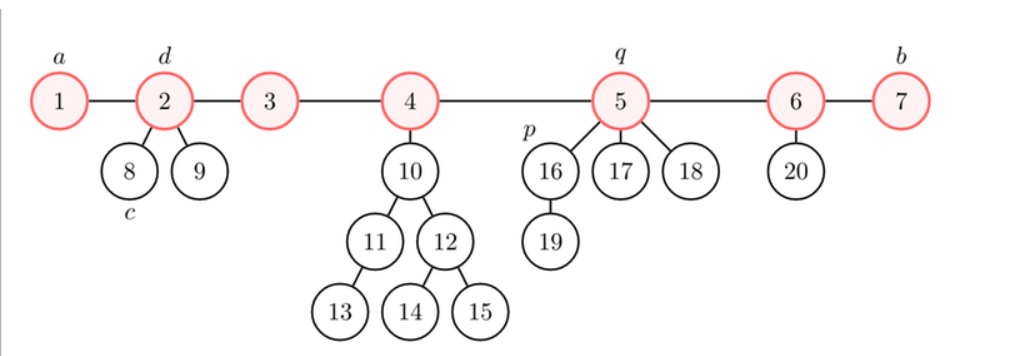
\includegraphics[width = 0.9\textwidth]{fig1.png}
\end{figure}

而森林的每个顶点均在直径上。设$x$所在部分的顶点为$r_1$。

(利用反证法)假设$a$不为直径端点,$s,t$为一条直径的两个端点。

不失一般性地可设$\text{dis}(x,s)\leq \dis(x,t)$。

则有
\begin{equation}
    \dis(x,a)>\dis(x,t) \Rightarrow \dis(r_1,a) > \dis(r_1,t) \Rightarrow \dis(s,a)>\dis(s,t).
\end{equation}

这与假设相悖,于是原命题得证。

同样根据定义可证以下引理:
\begin{lemma}
    对于树上一个直径的端点$a$, 记$b = \max_i(\dis(a,i))$, 则$a\rightarrow b$的路径必为直径。
\end{lemma}

于是只需按以上两个引理操作,分别以任意结点和第一次的结果进行两次树的遍历(推荐BFS遍历),每次寻找到距离根节点最远的结点,第二次的结果即是答案。

\subsection{适用性}
当题目所给为典型有根树状结构时,适合用算法一。如果是无根树(图论结构),适合用算法二。

\subsection{例6}
\href{https://leetcode.cn/problems/diameter-of-binary-tree/}{力扣-543. 二叉树的直径}
\subsubsection{Solution}
典型例题,给的数据结构为树,适用于算法一。
\subsubsection{Code}
\lstinputlisting[language=c++]{Code_6.cpp}

\subsection{例7}
\href{https://codeforces.com/contest/1805/problem/D}{CodeForces-Round 862(Div2)-D}
\subsubsection{Solution}

此题较为灵活,分析可得显然直径的端点是首次被合入的对象。设$T_i$表示以$i$为根时的树。

显然第$k$轮将会合并满足$h(T_i) = k$的点,即连通区域减少$\text{count}(h(T_i)=k)$(第一次合并减少$\text{count}(h(T_i)=k)-1$)。

根据引理\ref{lemma-1},$h(T_i) = k$等价于距离直径一端点距离较大值为$k$。

也即$\max(\dis(i,s),\dis(i,t)) = k$。

于是我们可以先找到一组直径的端点$s,t$,即可计算$h(T_i)$。

根据所给条件适宜使用算法二。

\subsubsection{Code}
\inputcppfile{Code_7.cpp}

\subsection{例8}
\href{https://www.luogu.com.cn/problem/P3304}{洛谷-SDOI2013-直径}
这道题是上述引理的综合应用。

第一问略。第二问需要求取所有直径都经过的边数,为此我们可以先将一条直径求取出来。

(利用树 = 直径 + 森林的做法)记$s,t$为一条直径的两个端点,$r$是直径上一点,$T_r$是去除直径后以$r$为根节点的深度。

显然,当$\exists x $使得在树$T_r$中有$h(x) = \dis(x,s)$时,路径$s \rightarrow r$便不是所有直径都经过的边的一部分,对于端点$t$此结论也成立。
\begin{lemma}
    对于上述描述的$x$,若存在,必有
    \begin{equation}
        h(x) = h(T_r) = \min(\dis(r,s),\dis(r,t)).
    \end{equation}
\end{lemma}

\emph{证明:}
使用反证法,证明如果不满足上述情况必有假设``$s,t$为直径的两个端点''断言为假即可。

记\begin{equation}
    f(v) = \max_{\dis(u,v) = h(T_u)}(\dis(u,v)), v \in \{s,t\}.
\end{equation}
于是
\begin{equation}
    \ans = \abs(f(s) - f(t)).
\end{equation}

上述算法在下图将会遇到特例,需要进行特别判定:
\begin{figure}[H]
    \centering
    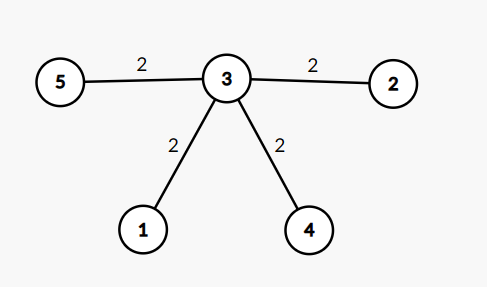
\includegraphics[width = 0.9\textwidth]{fig2.png}
\end{figure}

\subsubsection{Code}
\inputcppfile{Code_8.cpp}

\section{最近公共祖先问题}
两个结点的最近公共祖先为公共结点中深度最低的结点,记为$\lca(u,v)$。

性质:
\begin{enumerate}
    \item $\lca(u,v) = u$, 当且仅当$u$是$v$的祖先。
    \item 对于点集$A,B$, $\lca(A\cup B) = \lca(\lca(A),\lca(B))$.
    \item $\dis(u,v) = h(u)+h(v) - 2*h(\lca(u,v))$.
\end{enumerate}

\subsection{朴素算法}
记$\fa(x)$为结点$x$的根节点,根据性质1,可以推出转移方程式:
\begin{equation}
    \lca(u,v) = \begin{cases}
        u,                   & u = v       \\
        \lca(\fa(u),v),      & h(u)> h(v)  \\
        \lca(u,\fa(v)),      & h(u)< h(v)  \\
        \lca(\fa(u),\fa(v)), & h(u) = h(v)
    \end{cases}
\end{equation}

预处理复杂度$O(n)$, 单次查询复杂度为$O(h(T))$.
\subsubsection{例9}
\href{https://leetcode.cn/problems/lowest-common-ancestor-of-a-binary-tree/}{力扣-236. 二叉树的最近公共祖先}
\par\textbf{Code}\par
\inputcppfile{Code_9.cpp}

\subsection{倍增算法}
\subsection{子问题一:二进制转换}
首先先思考一个子问题:对于一个整数$x$,如何将其转换为二进制?

对于这个问题,朴素的做法是依次除2,即利用表达式
\begin{equation}
    \text{binary\_str}(x) = \begin{cases}
        \text{binary\_str}(x/2) + \text{`0'}, & x\%2 = 0 \\
        \text{binary\_str}(x/2) + \text{`1'}, & x\%2 = 1
    \end{cases}
\end{equation}
实践中,为了避免从字符串首部插入导致复杂度提升,常常先将字符插入至尾部,最后再进行翻转。
尽管如此,单次求取$x/2$常数还是比较大(较比于加减法和乘法)。

如果我们预处理数列$\{2^0,2^1,...,2^k\},  k \leq  \lfloor \log_2(n)\rfloor$的值,
于是可有
\begin{equation}
    \text{binary\_str}(x) = \begin{cases}
        \text{`0'} + \text{binary\_str}(x),       & x< 2^k    \\
        \text{`1'} + \text{binary\_str}(x - 2^k), & x\geq 2^k
    \end{cases}
\end{equation}
依次减少$k$的值,便可以求出二进制每位的值。

\textbf{例10:转换二进制}
\inputcppfile{Code_10.cpp}

\subsection{思路}
上述子问题给出了一种可能性,对于具备二分性质的数列可以通过预处理$2^k$数列来降低多次询问复杂度。

现在我们考虑利用这种方法优化朴素最近公共祖先问题。

首先我们考虑当$h(u)\neq h(v)$的情况,不失一般性性地假设$h(u)>h(v)$,

于是必存在$x$使得$h(\fa^{x}(u)) = h(v)$,其中

\begin{equation}
    \fa^{x}(u) = \begin{cases}
        \fa^{x-1}(u), & x > 1  \\
        \fa(u),       & x = 1  \\
        u,            & x = 0.
    \end{cases}
\end{equation}

对于任意$k$, 根据二进制分解的原理有
\begin{equation}
    \fa^{x}(u) = \begin{cases}
        \fa^{x}(u),                  & h(\fa^{2^k}(u)) < h(u)   \\
        \fa^{x - 2^k}(\fa^{2^k}(u)), & h(\fa^{2^k}(u)\geq h(u)) \\
    \end{cases}
\end{equation}

如果对于任意结点$u$我们提前预处理$f^{2^k}(u)$的值,然后依次减小$k$的值即可。

单次查询复杂度: $O(\log(n))$, k 最大为$\lfloor \log(n) \rfloor $。

现在我们考虑当$h(u) = h(v)$时求最近公共祖先的操作,同理,必存在最小的$y$,使得$\fa^y(u) = \fa^y(v)$.

同理,根据二进制分解的原理, 对于$k$ 有
\begin{equation}
    \lca(u, v) = \begin{cases}
        \lca(u,v),                       & \fa^{2^k}(u) =  \fa^{2^k}(v)    \\
        \lca(\fa^{2^k}(u),\fa^{2^k}(v)), & \fa^{2^k}(u) \neq  \fa^{2^k}(v)
    \end{cases}
\end{equation}

最后需要考虑$\fa^{2^k}(u)$的维护:
\begin{equation}
    \fa^{2^k}(u) = \begin{cases}
        \fa(u),                            & k= 0      \\
        \fa^{2^{k - 1}}(\fa^{2^{k-1}}(u)), & k \geq 1.
    \end{cases}
\end{equation}

注意需要考虑对非法值,即$2^k > h(u)$时的处理, 一般考虑赋为定义域之外的数。

\subsection{例11}
\href{https://www.luogu.com.cn/problem/P3379}{P3379 【模板】最近公共祖先(LCA)}
模板题,按照模板写即可。
\inputcppfile{Code_11.cpp}

\section{线段树}
\subsection{概述}

定义:将区间信息存储在结点的一种数据结构。其支持的操作为
\begin{enumerate}
    \item 区间修改,将区间$[L,R]$修改为新值。
    \item 区间查询,查询区间$[L,R]$的信息。
\end{enumerate}

\subsection{操作需要满足的条件}
线段树基于分治的原理。其维护的信息(统称操作)都需要满足以下条件:

\begin{enumerate}
    \item 操作必须是二元的。
    \item 操作必须满足结合律。
    \item 操作必须有幺元。
\end{enumerate}

几个满足线段树操作的例子:加减法、最大值、最小值、GCD、LCM等。

\subsection{结构}
常用的线段树满足以下性质:

\begin{enumerate}
    \item 线段树是一颗完整二叉树。
    \item 线段树的根节点编号为1,维护区间$[1,n]$的信息。
    \item 对于区间$[1,n]$,线段树的叶子结点从左往右依次维护$[1,1],[2,2]...,[n-1,n-1],[n,n]$的信息。
    \item 对于线段树的每个中间结点,设该节点维护区间$[x,y]$的信息,则其左儿子维护区间$[x,  \lfloor \frac{x+y}{2}\rfloor]$的信息,右儿子维护区间$[\lfloor \frac{x+y}{2} \rfloor +1,y]$的信息。
    \item 线段树采取堆式存储,也即对于编号$x$,其左儿子编号为$2x$,右儿子编号为$2x+1$.
\end{enumerate}

\subsection{性质}
\textbf{注意:这里的$n$指的是区间长度而不是常见的树的结点个数。}

\begin{lemma}
    线段树不存在两个结点不同但编号一样。
\end{lemma}
\emph{证明}:
假设存在两个结点编号均为$x$,所以其均为$\lfloor x/2 \rfloor $的子节点,且根据奇偶性可以判定其属于左儿子还是右儿子。

因此这两个结点是同一个结点,QED。


\begin{lemma}
    线段树的结点个数小于等于$2n-1$。
    \label{lemma-2}
\end{lemma}

\emph{证明}:

观察可得递推式
\begin{align*}
    f(n) = \begin{cases}
        2f(n/2) + 1, & \text{n是奇数,} \\
        f((n-1)/2) + f((n+1)/2) + 1, & \text{n是偶数.} 
    \end{cases}
\end{align*}

使用归纳法证明。
当$f(1) = 1, f(2) = 3$均成立。

考虑$f(n)$, 

当$n$为偶数时,$f(n) \leq 2\times(n/2\times2-1) + 1 \Leftrightarrow f(n) \leq 2n-1.$

当$n$为奇数时,$f(n) \leq (n-1)/2*2 - 1 + (n+1)/2*2 - 1 + 1 \Leftrightarrow f(n)\leq 2n-1.$.

均成立,QED.



\begin{lemma}
    线段树编号最大值小于$4n$。
\end{lemma}

\emph{证明}:

线段树深度最大不超过$2^{\lceil \log(n) \rceil}$,因此最大编号不超过

\begin{equation*}
    1 + 2 + 4 + .... + 2^{\lceil \log(n) \rceil}
\end{equation*}

即为$2^{\lceil \log(n) \rceil+1} < 2^{\log(n)+2} = 4n$.


\begin{lemma}
    线段树的高度不超过$O(\log(n))$.
\end{lemma}

\emph{证明}:由性质\ref{lemma-2}和完全二叉树的性质可证。-

\subsection{PURQ 数据结构}
PURQ —— "Point update range query", 也即单点修改,区间查询。

首先要构建线段树,开4倍空间采取递归建树即可。

其次是区间查询,

设$e$为查询信息的幺元,$\circ$为查询信息合并的操作。

要查询的区间为$[L,R]$, 当前所在叶节点维护的区间为$[l,r]$,信息为$\Inf(l,r)$.

有以下递推式:
\begin{align*}
    Q(L,R,l,r) = \begin{cases}
        \Inf(l,r) , & [l,r] \subseteq [L,R] \\
        e, & [l,r] \cap [L,R] = \emptyset \\
        Q(L,R,l,(l+r)/2) \circ Q(L,R,(l+r)/2+1,r), & \Else 
    \end{cases}  
\end{align*}

以上三种情况的条件也称为完全覆盖、不相交、部分覆盖。

单点更新和区间查询类似,见源代码。

\subsubsection{例13}
模板题,需要注意区间关系的判断条件。
\href{https://leetcode.cn/problems/range-sum-query-mutable/description/}{力扣-307. 区域和检索 - 数组可修改}
\inputcppfile{Code_13.cpp}

\subsection{RURQ 数据结构}
RURQ —— "Range update range query" 数据结构, 即区间修改,区间查询。

思考区间修改的问题,如果每次都去修改区间内的数据将会复杂度难以承受。

而如果只保存此次操作,改变对应结点的信息,便可以大大降低复杂度。

懒惰标记(lazy propagation)是优化区间更新的方法,其思想便是存储每次操作的结果,数组的更新只在进入到相应区间时发生。

懒惰标记维护的操作集合$F$需要满足以下条件,
\begin{enumerate}
    \item $F$含有单位变换$e$,使得$e(x) = x$.
    \item $F$中的元素是可复合的,也即对于$f,g\in F$,必有$f \circ g  \in F$.
    \item 对于维护信息的操作$\cdot$, $F$中的元素是可分配的。也即对于$f \in F$, $f(x\cdot y) = f(x)\cdot f(y)$。
\end{enumerate}

具体编程实现见例题。

\subsubsection{例14}
\href{https://www.luogu.com.cn/problem/P3372}{洛谷 - P3372 【模板】线段树 1}

需要维护的操作为区间求和,记$\text{lazy}(i)$表示线段树结点$i$未对子树更新部分。

一旦查询或更新到相应区间,$\text{lazy}(i)$存储的更新应该同步向下传递,

而本结点的标记清空,并且递归结束后需要更新该区间维护的信息。

\textbf{代码:}
\inputcppfile{Code_14.cpp}

\subsection{例15}
\href{https://www.luogu.com.cn/problem/P3373}{洛谷 - P3373 【模板】线段树 2}

与上述题目不同的是需要考虑操作的定义。

考虑操作$f(a,b,x) = (x + a)b$(先加后乘), 则
\begin{align*}
    f(c,d,f(a,b,x)) &= (f(a,b,x)+c)d \\
    &= ((x+a)b + c)d \\
    &= (x+a + c/b)bd \\ 
    &= f(a+c/b,bd,x)
\end{align*}

若$b = 0$,此时便不满足区间更新所需的第二条性质。

尽管我们可以通过约定此时$c/b = 0$使其满足该性质,然而对于$c/b$这部分的小数仍然是我们不希望得到的(不易维护)。

因此我们考虑定义$f(a,b,x) = ax+b$(先乘后加), 则
\begin{align*}
    f(c,d,f(a,b,x)) &= f(c,d,ax+b) \\
    &= acx + bc+d \\
    &= f(ac,bc+d) 
\end{align*}

此操作具备良好的性质,便于维护。

\textbf{代码}:
\inputcppfile{Code_15.cpp}

\subsection{线段树求解lca问题}
\subsubsection{子问题:RMQ问题}
RMQ——"Range Minimum/Maximum Query",区间最大/最小值查询。

无修改,直接用RQ数据结构维护即可(甚至不需要PU)。

\subsubsection{例16}
板子题。
\href{http://poj.org/problem?id=3264}{Balanced Lineup}

\textbf{代码:}
\inputcppfile{Code_16.cpp}
  
\subsubsection{思路}
首先我们需要介绍一棵树的欧拉序列。

定义:考虑一棵树的dfs遍历(最后要回到根节点),每遇到一个结点(无论是否是回溯的)便将序号其添加到序列中,最后得到的序列便是欧拉序列。这里的序号等于将第一次遇到该结点的时刻排序后的次序。


\begin{lemma}
    一棵树的欧拉序列长度为$2n-1$.($n$是结点个数。)
\end{lemma}

\emph{证明}:

采取归纳法,当$n = 1$时,欧拉序列长度为1,成立。

考虑一个子树$T_r$的根节点$r$, 设其子树为$T_1,T_2,...,T_l$, 

记函数$f(T_r)$为子树欧拉序列长度,$\text{c}(T_r)$为子树的大小,

从$r$出发回到$r$过程中经过$r$的次数为$l+1$.因此最后欧拉序列长度为
\begin{align*}
    f(T_r) & = \displaystyle \sum_{i = 1}^{l} f(T_i) + l + 1 \\
    &= \displaystyle \sum_{i = 1}^{l} (2c(T_i)-1) + l + 1\\
    &= 2(c(T_r)-1) - l + l + 1  \\
    &= 2c(T_r) - 1
\end{align*}

于是原命题得证。

\begin{lemma}
    对于树上两点$u,v$, $u,v$的最近公共祖先是欧拉序列中$u,v$对应位置(如果有多个,任取一个)组成的区间中的最小值。
\end{lemma}

\emph{证明}:
首先dfs的过程中对于每一条边最多经历2次,其次最近公共祖先必在上述区间中。

令$r$为满足上述性质的结点,若$r$不为$u,v$的最近祖先,则$r->\lca(u,v)$将会被遍历至少3次($r->u, u->r,r->\lca(u,v)$)。

与dfs性质不符,因此原命题证明。

\subsubsection{例17}
\href{https://www.luogu.com.cn/problem/P3379}{洛谷-P3379 【模板】最近公共祖先(LCA)}
题面同例11,模板题,使用RMQ和线段树求解版本。

\textbf{Code}:
\inputcppfile{Code_17.cpp}

\section{树链剖分}
\subsection{概述}

定义:将整棵树剖分为若干条链状结构,使用其余的数据结构维护信息。

树链剖分有很多种,如重链剖分、长链剖分、实链剖分,未明确说明的情况下本文的树链剖分都特指重链剖分。

树链剖分在以下的操作场景种很有用:
\begin{enumerate}
    \item 更新结点$u$和$v$路径上的所有结点。
    \item 查询结点$u$到$v$路径上的和、最大值、最小值等符合\textbf{结合律}的函数值。
\end{enumerate}

\subsection{数据结构定义}

\begin{enumerate}
    \item 重儿子:儿子结点中子树最大的一个。
    \item 轻儿子:非重儿子的儿子。
    \item 重边:连接一个结点和其重儿子的边。
    \item 轻边:连接一个结点和其任意轻儿子的边。
    \item 重链:由重边组成的路径,通常将只有没有重边相连的叶子结点也视为一条重链。
    \item 重链头: 一条重链中深度最低的结点, 记$\top(u)$表示结点$u$所在的重链的重链头。
    \item 轻链:由轻边组成的路径。
\end{enumerate}

\subsection{性质}
\begin{lemma}
    对于任意结点$x$和其祖先结点$y$,从$x->y$的路径中经过轻边的个数不超过$O(\log(n))$.
    \label{lemma-LCA-lightEdge}
\end{lemma}

\emph{证明}:

假设$u->v$是其经过的一条轻边,其中$u$是$v$的父亲结点。

根据定义,$u$必存在一重儿子$v'$, 且$\size(T_v')\geq \size(T_v)$。

因此$\size(T_u) \geq 2\size(T_v)$.

假设$l$表示$u->v$经过轻边的条数,根据上述迭代过程,则有

\begin{align*}
    \size(T_y) \geq 2^{l} \size(T_x) &\Leftrightarrow l \leq \log(\size(T_y)/\size(T_x)) \\
    &\Leftrightarrow l \leq O(\log(n)).
\end{align*}

\begin{lemma}
    对于树上任意结点$x$和$y$,从$x->y$的路径中经过轻边的个数不超过$O(\log(n))$.
\end{lemma}

\emph{证明}:

假设$r = \lca(x,y)$, 因此$x->y = x->r->y$. 

根据引理\ref{lemma-LCA-lightEdge}, $x->r, r->y$均为$O(\log(n))$,原命题得证。

\subsection{树链剖分解决lca问题}
\subsubsection{思路}
分析可得lca新的递推表达式:

不失一般性,这里约定$h(\top(u)) \geq  h(\top(v))$,可得$\lca(u,v)$在不同条件下的递推式:
\begin{numcases}{}
    u,  \top(u) = \top(v) \land h(u)\leq h(v) \nonumber \\ 
    v,  \top(u) = \top(v) \land h(u) > h(v) \nonumber \\
    \lca(\top(\fa(u)),v),  \top(u)\neq \top(v) \label{eq_lca1}
\end{numcases}

$\top(u)$的更新递推式如下:
\begin{align*}
    \top(u) = \begin{cases}
        \top(\fa(u)),  & u\text{是重儿子}, \\ 
        u, & u \text{是轻儿子}.
    \end{cases}
\end{align*}

\subsubsection{复杂度分析}
预处理$\top$等必要函数映射为$O(n)$.

分析递推表达式,执行$\ref{eq_lca1}$的次数等于$u,v$之间路径轻边的个数,为$O(\log(n))$.

因此单次查询$\lca(u,v)$复杂度为$O(\log(n))$.

\subsubsection{例12}
\href{https://www.luogu.com.cn/problem/P3379}{洛谷-P3379 【模板】最近公共祖先(LCA)}

题面同例11, 模板题,使用上述式子递推即可,相较于倍增法,使用树链剖分的常数较小。

代码:
\inputcppfile{Code_12.cpp}

\subsection{树链剖分与线段树}

如果规定dfs每次必须先走重儿子,那么每条重链的结点在DFS序中将是连续的。

那么对于每条重链上的信息,我们可以使用线段树维护,最终查询$u->v$的复杂度为$O(n\log^2(n))$.

\subsubsection{例18}
\href{https://cses.fi/problemset/task/2134/}{CSEC-Path Queries II}

模板题,只需要维护简单的路径求和。

\textbf{注:}这题最后一个测试点TLE了,经过长达几个小时的DEBUG,总结出以下特性:

\begin{enumerate}
    \item endl速度及其缓慢,应该严格限制。
    \item auto lambda表达式对于运行速度的影响不大。
    \item 关于左移位和右移位理论上会增加速度,但是通常编译器可以优化,因此影响不大。
    \item scanf速度慢于加了读入优化的cin。
\end{enumerate}

\inputcppfile{Code_18.cpp}

\section{参考资料}
 [1]. \href{https://oi-wiki.org/graph/tree-diameter/}{OI-wiki}

[2]. \href{https://www.geeksforgeeks.org/diameter-of-a-binary-tree/}{Geeksforgeeks}

[3]. \href{https://codeforces.com/blog/entry/101271}{CodeForces-Tutorial}

[4]. \href{https://blog.csdn.net/Q_M_X_D_D_/article/details/89924963?spm=1001.2101.3001.6650.1&utm_medium=distribute.pc_relevant.none-task-blog-2%7Edefault%7ECTRLIST%7ERate-1-89924963-blog-81060586.235%5Ev28%5Epc_relevant_t0_download&depth_1-utm_source=distribute.pc_relevant.none-task-blog-2%7Edefault%7ECTRLIST%7ERate-1-89924963-blog-81060586.235%5Ev28%5Epc_relevant_t0_download&utm_relevant_index=2}{CSDN论坛}

[5]. 算法导论(第三版)

[6]. \href{https://en.wikipedia.org/wiki/Segment_tree}{Wikipedia}

[7]. \href{https://atcoder.github.io/ac-library/production/document_en/lazysegtree.html}{AC Library}

\end{document}
